\noindent
\section{Importance of the editor}
\label{editor_imp}

Results from the previous section suggests that given the reviewer history and the related topic, our algorithm is able to correctly recommend a set of reviewers. It might therefore be tempting to believe that a peer-review system can be made to function without even the intervention of the editor. However, we would like to point out that this is not the case and our system simply recommends a set of reviewer groups to the editor from which (s)he has to use his/her expertise and knowledge to choose the most appropriate group. In fact the intervention of the editor to select the reviewer group for each paper is critical to the performance of our scheme in the long run. To illustrate this, we perform the following experiment. The multi-refereed papers are sorted based on their date of submission. The reviewer history for each referee is included till the point of submission of the first multi-refereed paper. For each paper our system recommends a set of reviewer groups; if we consider no editor intervention in our system, the top ranked (according to fitness score) reviewer group is selected from the set of recommended groups and the 
reviewer history updated accordingly. Note that for our original system, we assumed the editor selected the correct set of reviewers and the reviewer history was updated following the original assignment. Also since, in this simulation settings, we do not know whether the reviewers would have actually accepted or rejected the paper, we flag the paper as accepted with a probability proportional to the current average accept ratio of the assigned referees. The system is allowed to evolve following the above mentioned way.   

\begin{figure}
\centering
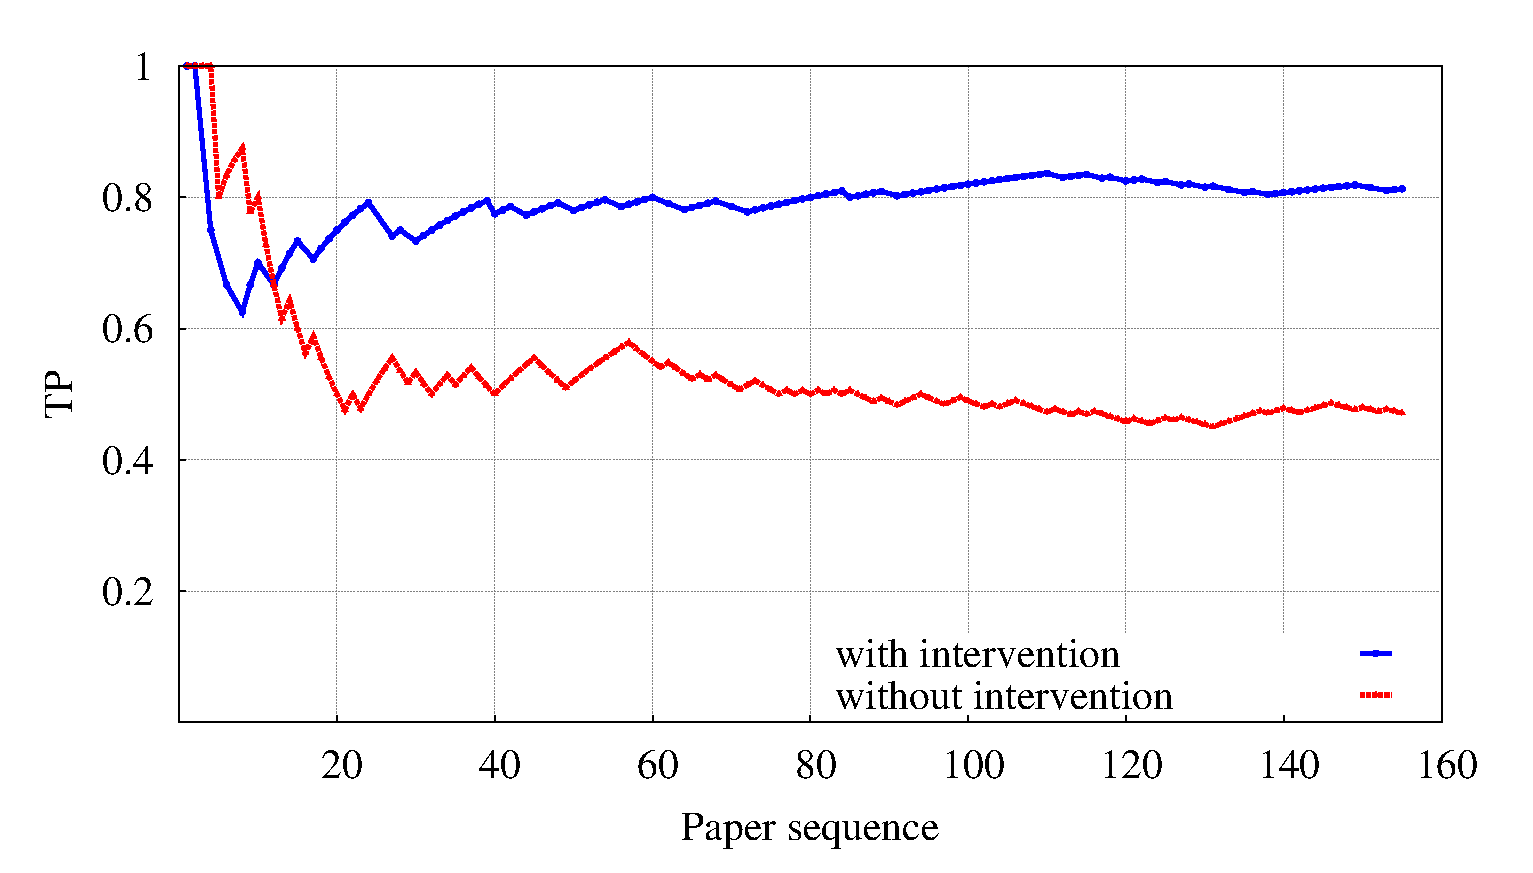
\includegraphics[scale = 0.26]{./texfiles/Chapter_4/cikm_17/figures/G_A_comp.eps}
\caption{\label{fig:ed_imp}True positive value at each point of recommendation of the top 25 percentile (based on citation) accepted papers for JHEP dataset. 
The papers are sorted by date of submission and x-axis denotes the paper number in the sequence.}
\vspace{4mm}
\end{figure}
\medskip

We now consider the top 25 percentile papers (based on citation) and sort them according to the date of submission. The simulation setup above is then used to recommend a set of reviewer groups. In figure~\ref{fig:ed_imp} we plot the TP value for each paper sorted according to their submission dates. Specifically, we calculate the fraction of correct recommendations at the point of every new submission for both the original system (with editor intervention) and the simulation system (without intervention). We observe that the performance of the system without intervention degrades alarmingly over time compared to the original system. The above results indicate that the expert intervention of the editor in choosing the reviewer groups is extremely important toward proper functioning of the peer-review system. 